\documentclass[a4paper,UKenglish,cleveref, autoref, thm-restate]{qlinhta}
\usepackage{amsmath}
\usepackage{algorithm}
\usepackage{algpseudocode}
\usepackage{booktabs}
\usepackage{longtable}
\setlength{\tabcolsep}{5pt}
\renewcommand{\arraystretch}{1.5}
\usepackage{tikz}
\usepackage{subcaption}
\usepackage{amsmath}
\usepackage{amsfonts}
\usepackage{amssymb}
\usetikzlibrary{shapes.geometric, arrows}
\tikzstyle{startstop} = [rectangle, rounded corners, 
minimum width=3cm, 
minimum height=1cm,
text centered, 
draw=black, 
fill=red!30]

\tikzstyle{io} = [trapezium, 
trapezium stretches=true, % A later addition
trapezium left angle=70, 
trapezium right angle=110, 
minimum width=3cm, 
minimum height=1cm, text centered, 
draw=black, fill=blue!30]

\tikzstyle{process} = [rectangle, 
minimum width=3cm, 
minimum height=1cm, 
text centered, 
text width=3cm, 
draw=black, 
fill=orange!30]

\tikzstyle{decision} = [diamond, 
minimum width=3cm, 
minimum height=1cm, 
text centered, 
draw=black, 
fill=green!30]
\tikzstyle{arrow} = [thick,->,>=stealth]
\bibliographystyle{plainurl}

\title{Revision note: Artificial Intelligence}

\titlerunning{Revision note: Artificial Intelligence}

\author{Quyen Linh TA}{University Paris Dauphine, PSL}{quyen-linh.ta@dauphine.eu}{}{}

\authorrunning{Quyen Linh TA}


\begin{document}

\maketitle

\tableofcontents
\section{Search Problems}
Search algorithms stand at the heart of numerous aspects in Artificial Intelligence (AI). They act as the structural backbone for most systematic methods used to traverse and explore different possible alternatives in a problem space. Four main categories of search algorithms. These can be differentiated along two dimensions:

\begin{itemize}
    \item \textbf{Informed vs Uninformed:} Uninformed search algorithms, often called blind search, function without any additional, problem-specific information. On the other hand, informed search algorithms, also known as heuristic search, leverage task-specific information to enhance the efficiency of the search process.
    \item \textbf{Any-Path vs Optimal:} Any-path searches stop at the discovery of any solution, regardless of its quality. Optimal searches, however, strive to find the best possible solution, considering the quality of the path.
\end{itemize}
\subsection{Terminology}
\subsubsection{Tree and Graph}
The search strategies that we will investigate operate on trees and graphs. Thus, it is crucial to understand the associated terminologies:

\begin{itemize}
    \item A \textbf{tree} consists of nodes (or vertices) and links (or edges) connected in a way that avoids loops (or cycles).
    \item A tree begins at the \textbf{root node}. Every node, apart from the root, has a singular \textbf{parent} (or direct ancestor). Following this line of ancestry through the parent nodes repeatedly, we can identify all \textbf{ancestors} of a node.
    \item Each node, barring the \textbf{terminal nodes} (or leaf nodes), possesses one or more \textbf{children} (or direct descendants). Likewise, by traversing through the child nodes, we can identify all \textbf{descendants} of a node.
\end{itemize}

\begin{figure}[H]
    \centering
    \begin{minipage}{0.45\textwidth}
        \centering
        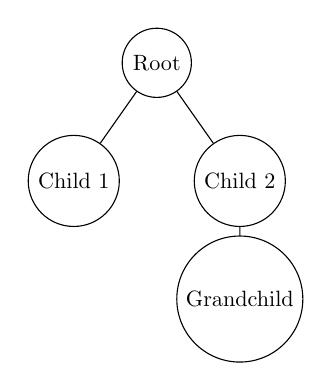
\begin{tikzpicture}[sibling distance=6em, every node/.style = {shape=circle, scale=0.8, draw, align=center}]]
            \node {Root}
                child { node {Child 1} }
                child { node {Child 2} 
                    child { node {Grandchild} } };
        \end{tikzpicture}
        \caption{A Tree}
    \end{minipage}
    \hfill
    \begin{minipage}{0.45\textwidth}
        \centering
        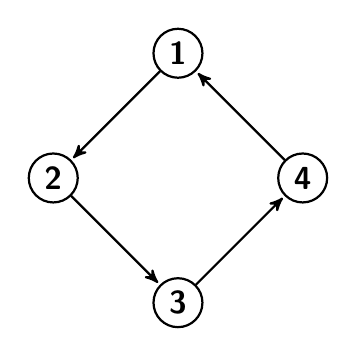
\begin{tikzpicture}[->,>=stealth',shorten >=1pt,auto,node distance=2.8cm, thick,main node/.style={circle, scale=0.8, draw,font=\sffamily\Large\bfseries}]
            \node[main node] (1) {1};
            \node[main node] (2) [below left of=1] {2};
            \node[main node] (3) [below right of=2] {3};
            \node[main node] (4) [below right of=1] {4};
            \path[every node/.style={font=\sffamily\small}]
            (1) edge node [left] {} (2)
            (2) edge node [right] {} (3)
            (3) edge node [right] {} (4)
            (4) edge node [left] {} (1);
        \end{tikzpicture}
        \caption{A Graph}
    \end{minipage}
\end{figure}

A graph is also a set of nodes connected by links but where loops are allowed and a node can have multiple parents. We have two kinds of graphs to deal with: directed graphs, where the links have direction (akin to one-way streets). And, undirected graphs where the links go both ways. Think of an undirected graph as shorthand for a graph with directed links going each way between connected nodes.\\

In many circumstances, the nodes of a graph may signify abstract descriptions of a state of the world. For instance, in a block-stacking scenario, nodes could represent different arrangements of blocks, while the edges could signify actions that transition between these states.\\

\subsubsection{Problem solving paradigm}

A path through the graph or tree, from a starting node to a goal node, can be seen as a strategic plan to achieve a desired state from a known initial state. These types of graphs hold considerable interest in AI, where problem-solving often involves graph searching.\\

To apply this approach, we must define the \textbf{states}, \textbf{actions}, and \textbf{goal} tests. A state should comprehensively represent all relevant aspects of the problem to solve, including only necessary details. For example, when planning an economical round-the-world flight itinerary, knowing the airport's identity suffices over its address, which would be relevant only when planning the route from the hotel to the airport.\\

We also make certain assumptions about the actions. We assume they are deterministic, meaning the state after an action is well-defined and certain. Furthermore, we assume that actions are discrete, excluding the need to represent the state during an action.\\

Importantly, our focus typically lies on a goal test, not just a single goal state. For instance, we might aim to reach any city in Germany instead of specifically Frankfurt. Or, when proving a theorem, we aim to establish a fact in our existing knowledge base, with any final set of facts containing the desired fact serving as a proof. \\

In principle, we could start with multiple starting states, for instance, if there's uncertainty about the initial state. However, at this stage, we will not delve into the issues of uncertainty in the starting state or the action outcomes.\\

\subsubsection{Tree Search and Graph Search}

Trees can be considered a special kind of directed graphs where the links, though not always represented by arrows, have a clear direction. Two distinguishing properties of trees within the broader category of directed graphs are that they lack cycles and every node has a single parent, except for the root.\\

\begin{figure}[H]
    \centering
    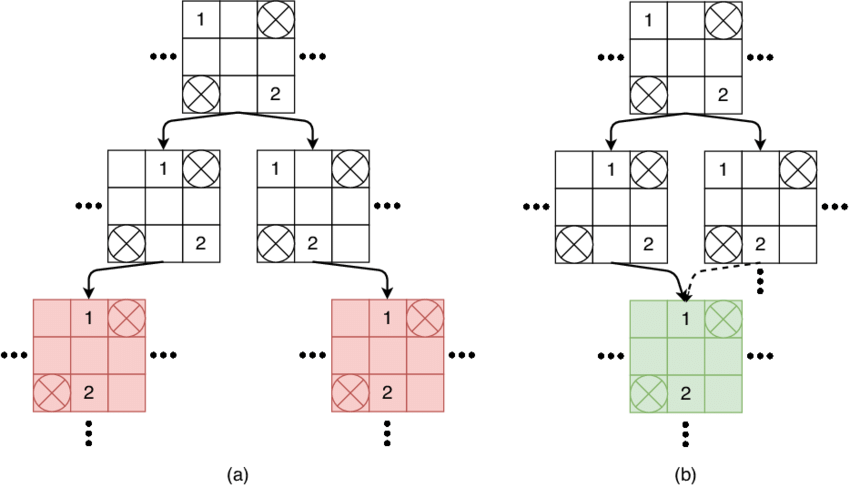
\includegraphics[width=13cm]{QPP/images/Differences-between-Tree-Search-a-and-Graph-Search-b-approaches.png}
    \caption{Differences between tree search $(a)$ and graph search $(b)$}
    \label{fig:tree_graph_search}
\end{figure}

In the context of search, cycles can be detrimental, as they can lead to endlessly recurring paths without progress. Consequently, when tasked with a graph search problem, we can translate it into an equivalent tree search problem by implementing two strategies.\\

Firstly, we can transform undirected links into bidirectional ones, effectively creating two directed links. More importantly, we can avoid considering paths with loops or, to further optimize the search process, avoid revisiting any node. This approach ensures that our search mimics a tree structure, thereby avoiding the potential pitfalls associated with cycles in graphs.\\

Let's illustrate the conversion of a graph to a tree with an example, figure \ref{fig:conversion_tree}. Consider a graph where $\mathcal{S}$ is our starting point and we aim to find a path to $\mathcal{G}$. As we traverse this graph, we form links from each node to all other connected nodes that wouldn't form a cycle, and we stop once we reach $\mathcal{G}$. This process produces a tree where each leaf node corresponds to a unique non-looping path in the original graph, beginning at $\mathcal{S}$.\\

Despite our efforts to prevent loops, we might still find duplicate nodes in our tree (highlighted in color), these are nodes that can be reached via different non-looping paths. This duplication suggests that our tree search might perform redundant work.\\

The balance between effort spent on preventing loops and reducing extra visits to nodes is a critical topic that we'll delve into later when we discuss various search algorithms.\\

To navigate these complexities, it's crucial to understand the difference between a 'state' and a 'search node':
\begin{itemize}
    \item A \textbf{state} represents a specific configuration of the real world (or our model of it). We're operating under the assumption of a "real" state graph that we're searching through. This graph might not be explicitly defined within our computational model but rather implied by the actions. We also assume that the same real-world state can be reached via multiple paths, or sequences of actions.
    \item A \textbf{search node}, in contrast, is a data structure used by the search algorithm. While conducting a search, the algorithm generates an explicit tree of search nodes. Each node corresponds to some state but not uniquely. Each node also signifies a path from the start state to its associated state, owing to the tree-structure generation of the search algorithm. Hence, when we return a node, we're essentially returning a path.
\end{itemize}

\begin{figure}[h]
    \centering
    \begin{subfigure}{.5\textwidth}
        \centering
        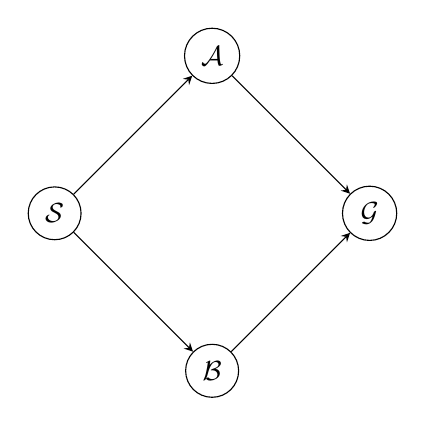
\begin{tikzpicture}
            \node[draw, circle] (s) at (0,0) {$\mathcal{S}$};
            \node[draw, circle] (a) at (2,2) {$\mathcal{A}$};
            \node[draw, circle] (b) at (2,-2) {$\mathcal{B}$};
            \node[draw, circle] (g) at (4,0) {$\mathcal{G}$};
            \draw[->,>=stealth] (s) -- (a);
            \draw[->,>=stealth] (s) -- (b);
            \draw[->,>=stealth] (a) -- (g);
            \draw[->,>=stealth] (b) -- (g);
        \end{tikzpicture}
        \caption{A simple graph from $\mathcal{S}$ to $\mathcal{G}$}
    \end{subfigure}%
    \begin{subfigure}{.5\textwidth}
        \centering
        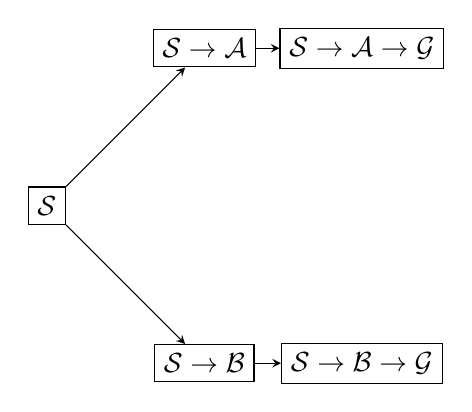
\begin{tikzpicture}
            \node[draw, rectangle] (s) at (0,0) {$\mathcal{S}$};
            \node[draw, rectangle] (sa) at (2,2) {$\mathcal{S}\to\mathcal{A}$};
            \node[draw, rectangle] (sb) at (2,-2) {$\mathcal{S}\to\mathcal{B}$};
            \node[draw, rectangle] (sag) at (4,2) {$\mathcal{S}\to\mathcal{A}\to\mathcal{G}$};
            \node[draw, rectangle] (sbg) at (4,-2) {$\mathcal{S}\to\mathcal{B}\to\mathcal{G}$};
            \draw[->,>=stealth] (s) -- (sa);
            \draw[->,>=stealth] (s) -- (sb);
            \draw[->,>=stealth] (sa) -- (sag);
            \draw[->,>=stealth] (sb) -- (sbg);
        \end{tikzpicture}
        \caption{The corresponding tree with no cycles}
    \end{subfigure}
    \caption{Graph to tree conversion}
    \label{fig:conversion_tree}
\end{figure}

\subsection{Classes of Search}
\begin{table}[h]
\centering
\begin{tabular}{|p{4cm}|p{4cm}|p{6cm}|}
\hline
\textbf{Classes} & \textbf{Name} & \textbf{Operation} \\
\hline
Uninformed, Any-path & Depth-first, Breadth-first & Look at all nodes in a specific order and stop when the first path to a goal state is found \\
\hline
Informed, Any-path & Heuristic algorithms & Exploit a task-specific measure of goodness to reach the goal more quickly or find a more desirable goal state \\
\hline
Uninformed, Optimal & Optimal algorithms & Guarantee finding the "best" path but do not use any information beyond what is in the graph definition \\
\hline
Informed, Optimal & Heuristic optimal algorithms & Guarantee finding the best path and exploit heuristic information to find the path faster than the uninformed methods \\
\hline
\end{tabular}
\caption{Classes of search algorithms}
\label{tab:search_classes}
\end{table}

\textbf{Example: Common Search Algorithm} The algorithm we will consider is based on the principle of maintaining a list of nodes, denoted as $Q$, where each node represents a partial path. We continuously pick a node from this list $Q$, inspect if it leads to the goal, and if not, we expand this path to its neighbors and add them back to the list $Q$. This is essentially the operation of our algorithm.\\

Importantly, we keep a record of the states we've visited and prevent their multiple entries into $Q$. This strategy is critical as it avoids potential loops, irrespective of the structure of the underlying graph, since a state can only be reached once. We will delve into the implications of this approach in later sections. \\

\begin{algorithm}
\caption{Solution: Common Search Algorithm}
\begin{algorithmic}[1]
\State Initialize $Q$ with search node $S$, set $Visited = \{S\}$
\While{$Q$ is not empty}
    \State Pick a node $N$ from $Q$
    \If{state($N$) is goal}
        \State \Return $N$ \Comment{Goal reached!}
    \EndIf
    \State Remove $N$ from $Q$
    \State Find all descendants of state($N$) not in $Visited$
    \For{each descendant}
        \State Create a one-step extension of $N$ to the descendant
    \EndFor
    \State Add the expanded paths to $Q$
\EndWhile
\end{algorithmic}
\end{algorithm}

The key questions, of course, are which entry to pick off of $Q$ and how precisely to add the new paths back onto $Q$. Different choices for these operations produce the various search strategies.

\begin{description}
\item[Visited] A state is considered "visited" when a path that reaches that state (i.e., a node that refers to that state) is added to Q. If the state exists in any node in Q, it has been visited. This holds true even if no path to that state has been removed from Q.

\item[Expanded] A state M is "Expanded" when a path to that state is removed from Q. At this point, the descendants of M are visited, and the paths to those descendants are added to Q.

\item[Heuristic] In general, a heuristic is a "rule of thumb" or a practical method not guaranteed to be optimal or perfect, but sufficient for the immediate goals. In the context of search algorithms, a heuristic may provide a way to guess which path could lead to a goal.

\item[Heuristic Function] A heuristic function is a function defined on a state (not on a path) that can be useful in guiding a search but doesn't guarantee to produce the desired outcome. Heuristic searches generally make no guarantees on shortest paths or best outcomes. Nonetheless, using heuristic functions may expedite the process of finding a goal, at least on average.

\item[Estimated Distance to Goal] If we can approximate the "distance" to a goal from the current node and prefer nodes closer to the goal, then there's a good chance that the search will end more quickly. This intuition is evident when considering "as-the-crow-flies" distance to guide a search in Euclidean space, but it generalizes to more abstract situations.
\end{description}

\begin{table}[h]
\centering
\begin{tabular}{|p{2cm}|p{3cm}|p{9.5cm}|}
\hline
\textbf{Information Used} & \textbf{Path Quality} & \textbf{Algorithms} \\
\hline
Uninformed & Any-path & Depth-first search, Breadth-first search, Depth-limited search, Iterative deepening depth-first search, Bidirectional search, D-Algorithm, B* Algorithm, AO* Algorithm, Constraint satisfaction search, AND-OR search trees \\
\hline
Informed & Any-path & Best-first search, Greedy best-first search, Hill-climbing search, Simulated annealing, Beam search, Genetic algorithms, Tabu search, Ant colony optimization, Particle swarm optimization, Stochastic diffusion search, Viterbi Algorithm \\
\hline
Uninformed & Optimal & Uniform-cost search, Dijkstra's Algorithm, Breadth-first search (if costs are identical), Bellman-Ford Algorithm, Floyd-Warshall Algorithm, V-optimal Algorithm, Lexicographic Breadth-First Search \\
\hline
Informed & Optimal & A* search, Iterative deepening A* (IDA*), Simplified Memory-Bounded A* (SMA*), Fringe Search, Recursive best-first search, Beam-Stack search, Branch and bound, Jump point search \\
\hline
\end{tabular}
\caption{Search Algorithms Classified by the Information Used and Path Quality}
\label{tab:search_algorithms_extended}
\end{table}


\begin{table}[h]
\centering
\begin{tabular}{|l|p{10cm}|}
\hline
\textbf{Environment Observability} & \textbf{Search Algorithms} \\
\hline
Fully Observable & Depth-First Search, Breadth-First Search, Uniform Cost Search, Greedy Best-First Search, A* Search \\
\hline
Partially Observable & Markov Decision Process based methods, Partially Observable Markov Decision Process (POMDP) methods, Monte Carlo Tree Search, Reinforcement Learning methods like Q-Learning \\
\hline
\end{tabular}
\caption{Search Algorithms categorized by environment observability}
\label{tab:observable_search}
\end{table}

In this Table \ref{tab:observable_search}, we classify search algorithms based on the observability of the environment. "Fully Observable" means that the complete state of the environment is known at each decision point, which is a basic assumption of classical search algorithms like Depth-First Search and A* Search.\\

In contrast, the "Partially Observable" category includes methods designed to handle uncertainty about the state of the environment. Techniques like Markov Decision Processes (MDPs), Partially Observable Markov Decision Processes (POMDPs), Monte Carlo Tree Search, and Reinforcement Learning methods like Q-Learning are included in this category. These algorithms can deal with situations where the full state of the environment is not known at each decision point, which adds a significant layer of complexity to the search process.\\

\section{Algorithms Modelling}
\subsection{Generic Tree Search and Graph Search}
The \texttt{TREE SEARCH} algorithm operates on problems where the state space can be represented as a tree. Here is how it works:

\begin{itemize}
\item The function takes as input a \texttt{problem} and a \texttt{strategy}. The \texttt{problem} represents the task that needs to be solved, while the \texttt{strategy} determines the rule for selecting the next node to be expanded.
\item The frontier, $\mathcal{F}$, is a data structure that holds all available nodes for expansion. Initially, it is populated with the initial state $\mathcal{S}$ of the problem.
\item The explored set, $\mathcal{E}$, is used to keep track of all nodes that have been expanded so far. Initially, this set is empty.
\item The algorithm operates in a loop, continually exploring until a solution is found, or there are no more nodes to expand. If the frontier is empty and no solution has been found, the problem has no solution and the function returns failure.
\item A leaf node $\mathcal{N}$ is chosen and removed from the frontier according to the strategy.
\item If the node $\mathcal{N}$ contains a goal state $\mathcal{G}$, the function has found a solution and returns it.
\item If it's not a goal state, the node is added to the explored set, and all its successors are added to the frontier. However, nodes are only added to the frontier if they are not already in the frontier or the explored set. This step avoids unnecessary repetitions and loops in the search.
\end{itemize}
\begin{algorithm}[H]
\caption{Tree Search}\label{alg:tree_search}
\begin{algorithmic}[1]
\Procedure{TREE SEARCH}{problem, strategy}
\State Initialize the frontier $\mathcal{F}$ using the initial state $\mathcal{S}$ of problem
\State Initialize the explored set $\mathcal{E}$ to be empty
\While{True}
    \If{$\mathcal{F}$ is empty}
        \State \Return failure
    \EndIf
    \State Choose a leaf node $\mathcal{N}$ and remove it from $\mathcal{F}$
    \If{$\mathcal{N}$ contains a goal state $\mathcal{G}$}
        \State \Return the corresponding solution
    \EndIf
    \State Add $\mathcal{N}$ to $\mathcal{E}$
    \State Expand the chosen node $\mathcal{N}$, adding the resulting nodes to $\mathcal{F}$
    \State Only if not in $\mathcal{F}$ or $\mathcal{E}$
\EndWhile
\EndProcedure
\end{algorithmic}
\end{algorithm}

The \texttt{GRAPH SEARCH} algorithm is similar to the \texttt{TREE SEARCH} algorithm but is adapted to handle problems where the state space can be represented as a graph. This is because graphs allow states to have multiple parents, leading to potential loops in the state space.

The primary difference between the two algorithms is the handling of the frontier. In \texttt{GRAPH SEARCH}, a node is only added to the frontier if it is not already present in the frontier or the explored set.

The rest of the steps in \texttt{GRAPH SEARCH} are similar to those in \texttt{TREE SEARCH}. These include initializing the frontier and the explored set, checking if the frontier is empty, choosing and removing a node from the frontier, checking if the node contains a goal state, and expanding the node.

In both algorithms, the choice of strategy significantly impacts the efficiency and completeness of the search. Different strategies include breadth-first, depth-first, uniform-cost, greedy best-first, A*, among others. Each strategy has different properties and is suited to different types of problems.
\begin{algorithm}[H]
\caption{Graph Search}\label{alg:graph_search}
\begin{algorithmic}[1]
\Procedure{GRAPH SEARCH}{problem, strategy}
\State Initialize the frontier $\mathcal{F}$ using the initial state $\mathcal{S}$ of problem
\State Initialize the explored set $\mathcal{E}$ to be empty
\While{True}
    \If{$\mathcal{F}$ is empty}
        \State \Return failure
    \EndIf
    \State Choose a leaf node $\mathcal{N}$ and remove it from $\mathcal{F}$ [depending on the strategy]
    \If{$\mathcal{N}$ contains a goal state $\mathcal{G}$}
        \State \Return the corresponding solution
    \EndIf
    \State Add $\mathcal{N}$ to $\mathcal{E}$
    \State Expand the chosen node $\mathcal{N}$, adding the resulting nodes to $\mathcal{F}$
    \State Only if not in $\mathcal{F}$ or $\mathcal{E}$
\EndWhile
\EndProcedure
\end{algorithmic}
\end{algorithm}

\subsection{Fully observable}
In a \textbf{fully observable environment}, the agent perceives the complete state of the environment at each point in time. This provides perfect information for the agent's decision-making process. Essential concepts in this context include:

\begin{itemize}
\item \textbf{State Space:} The complete set of all possible configurations of the environment. The size can range from small to extremely large.

\item \textbf{Deterministic vs. Stochastic:} In a deterministic environment, the outcome of an action is fixed and predictable. In contrast, a stochastic environment's action outcome is probabilistic.

\item \textbf{Search Algorithms:} Algorithms used to explore the state space and find a path from the initial state to a goal state. Examples include depth-first search, breadth-first search, and A* search.

\item \textbf{Optimal Policies:} A policy defines the action an agent should take in each state. An optimal policy maximizes the agent's expected reward over a sequence of states.

\item \textbf{Performance Measure:} Quantifies the agent's success at achieving its goal. In fully observable environments, the agent can perceive its actions' effect on the performance measure.

\item \textbf{Single-Agent vs. Multi-Agent:} Fully observable environments can contain a single agent or multiple agents. In multi-agent environments, one agent's actions can affect other agents' states.
\end{itemize}

\subsubsection{Uniform Cost Search}

\begin{itemize}
\item \textbf{Optimality:} Uniform Cost Search is optimal as it always expands the least-cost node. The optimality is guaranteed under the condition that the cost of each action to transition from one state to another is non-negative.
\item \textbf{Path Quality:} Uniform Cost Search ensures the optimal path, not just any path. It is because it systematically explores paths from the root, always expanding the path with the smallest total cost.
\item \textbf{Observable Environment:} Uniform Cost Search operates in a fully observable environment. It assumes complete knowledge of the problem domain and uses this knowledge to guide its search.
\item \textbf{Informed or Uninformed:} Uniform Cost Search is considered an uninformed (or blind) search method as it doesn't have any information about the goal's location; it uses only the information provided by the problem itself. It systematically explores the state space without using any heuristic function to estimate the cost from a state to a goal.
\end{itemize}

\begin{algorithm}[H]
\caption{Uniform Cost Search}\label{alg:uniform_cost_search}
\begin{algorithmic}[1]
\Function{UCS}{problem}
\State Initialize $\mathcal{N}$ with the initial state of the problem
\State Initialize $\mathcal{F}$ as a priority queue ordered by the path cost $g$, with $\mathcal{N}$ as the only element
\State Initialize the explored set $\mathcal{E}$ to be empty
\While{True}
    \If{$\mathcal{F}$ is empty} 
        \State \Return failure
    \EndIf
    \State $\mathcal{N}$, $c$ $\gets$ pop the lowest-cost node in $\mathcal{F}$
    \If{$\mathcal{N}$ meets the goal test}
        \State \Return the corresponding solution
    \EndIf
    \For{each $a \in \text{ACTIONS}(\mathcal{N})$}
        \State $\mathcal{C}$ $\gets$ RESULT($\mathcal{N}$, $a$)
        \State $c'$ $\gets$ $c$ + COST($\mathcal{N}$, $a$)
        \If{$\mathcal{C} \notin \mathcal{E} \cup \mathcal{F}$}
            \State Push $\mathcal{C}$ into $\mathcal{F}$
        \ElsIf{$\mathcal{C} \in \mathcal{F}$ with path cost $>$ $c'$}
            \State Replace that frontier node with $(\mathcal{C}, c')$
        \EndIf
    \EndFor
\EndWhile
\EndFunction
\end{algorithmic}
\end{algorithm}

Now breaking it down:
\begin{enumerate}
    \item The algorithm begins by initializing the node $\mathcal{N}$ with the initial state of the problem.
    \item It also sets up the frontier $\mathcal{F}$ as a priority queue, which is ordered by the path cost $g$. At this point, $\mathcal{N}$ is the only element in $\mathcal{F}$.
    \item It then creates an empty set $\mathcal{E}$ for the nodes that have been explored.
    \item The main part of the algorithm is a loop that continues until a solution is found or it's determined that no solution exists.
    \item The first step in each iteration of the loop is to check whether $\mathcal{F}$ is empty. If it is, that means there are no more nodes to explore, and the algorithm returns a failure.
    \item If $\mathcal{F}$ isn't empty, the algorithm removes the lowest-cost node and assigns it to $\mathcal{N}$.
    \item If $\mathcal{N}$ meets the goal test (i.e., it is a goal state), the algorithm returns the corresponding solution.
    \item The algorithm then goes through each possible action $a$ that can be applied to $\mathcal{N}$. For each action, it determines the resulting child node $\mathcal{C}$ and calculates the new cost $c'$.
    \item If $\mathcal{C}$ isn't in $\mathcal{E}$ or $\mathcal{F}$, it is added to $\mathcal{F}$.
    \item If $\mathcal{C}$ is already in $\mathcal{F}$ but the new path cost $c'$ is lower than the existing cost, the algorithm replaces the existing node in $\mathcal{F}$ with the new lower-cost node.
\end{enumerate}
\vspace{5pt}
These steps continue until a solution is found or all possibilities have been exhausted. This is how the Uniform Cost Search algorithm explores all possible states while always prioritizing the lowest-cost options first.

\begin{table}[H]
\centering
\begin{tabular}{|l|l|}
\hline
\textbf{Complexity Measure} & \textbf{Uniform Cost Search} \\
\hline
Time Complexity & $O(b^{C*/\varepsilon})$ \\
\hline
Space Complexity & $O(b^{C*/\varepsilon})$ \\
\hline
Optimal & Yes \\
\hline
Complete & Yes (if cost is finite) \\
\hline
\end{tabular}
\caption{Complexity of Uniform Cost Search. Here, $b$ is the branching factor, $C*$ is the cost of the optimal solution, and $\varepsilon$ is the minimum cost of any action. The time and space complexity are both $O(b^{C*/\varepsilon})$, accounting for the fact that there is always at least one level (the root) to be explored, in addition to nodes with costs up to and including $C*$. UCS is optimal and complete, as it will always find a solution if one exists and it guarantees the solution is optimal.}
\label{tab:ucs_complexity_detailed}
\end{table}

\hl{\textbf{N.B:} M. GILBERT write $O(b^{1 + C*/\varepsilon})$, the form $O(b^{C*/\varepsilon})$ is a simplified form of $O(b^{1 + C*/\varepsilon})$, assuming $C* > 0$ and $\varepsilon > 0$. In some cases, we write it as $O(b^{1 + C*/\varepsilon})$ to specifically denote that there is always at least one level (hence the $+1$ in the exponent) that needs to be explored, which refers to the root node.}

\paragraph*{Application}
We will use this simple weighted graph:

\begin{center}
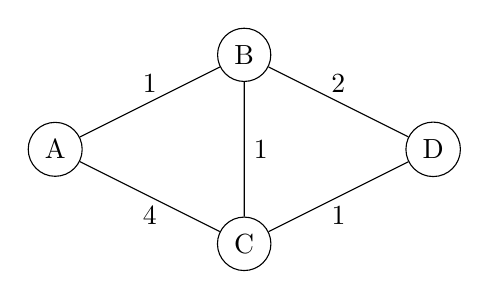
\begin{tikzpicture}[scale=0.6]
  \node[draw,circle] (A) at (0,0) {A};
  \node[draw,circle] (B) at (4,2) {B};
  \node[draw,circle] (C) at (4,-2) {C};
  \node[draw,circle] (D) at (8,0) {D};
  
  \draw (A) -- node[above] {1} (B);
  \draw (B) -- node[above] {2} (D);
  \draw (A) -- node[below] {4} (C);
  \draw (C) -- node[below] {1} (D);
  \draw (B) -- node[right] {1} (C);
\end{tikzpicture}
\end{center}

In this graph, each node represents a state, each edge represents an action that leads to a new state, and the numbers on the edges represent the cost of the action. Our goal is to find the path of least cost from A to D. The steps of the Uniform Cost Search algorithm execution are as follows:

\begin{enumerate}
  \item Initialize the frontier with the initial state A. The cost to reach A ($g(A)$) is 0.
  \item Expand node A, add all its neighbors to the frontier. Update the costs for each node: $g(B) = 1$, $g(C) = 4$.
  \item Choose the node from the frontier with the least cost, which is B. Expand B, update the costs: $g(C) = 2$, $g(D) = 3$.
  \item The node from the frontier with the least cost is now D, which is the goal node. Hence, the algorithm terminates.
\end{enumerate}

The path of least cost found by the algorithm is A-B-D, and the total cost is 3.

\subsubsection{Depth-First Search}

Depth-First Search (DFS) is another popular search algorithm used in problem-solving. Unlike UCS, DFS doesn't consider the cost of paths. It explores as far as possible along each branch before backtracking.

\begin{itemize}
\item \textbf{Optimality:} DFS is not optimal. It could find a solution, but not necessarily the least-cost solution.
\item \textbf{Path Quality:} DFS does not guarantee the quality of the solution, as it might not find the shortest path.
\item \textbf{Observable Environment:} Like UCS, DFS operates in a fully observable environment and assumes complete knowledge of the problem domain.
\item \textbf{Informed or Uninformed:} DFS is an uninformed search method as it doesn't have any information about the goal's location, it uses only the information provided by the problem itself. DFS explores the state space systematically without any heuristic estimation.
\end{itemize}

\begin{algorithm}[H]
\caption{Recursive Depth-First Search}\label{alg:recursive_dfs}
\begin{algorithmic}[1]
\Function{Recursive-DFS}{$\mathcal{N}$, problem}
    \If{$\mathcal{N}$ meets goal test}
        \State \Return $\mathcal{N}$
    \Else
        \For{each $a \in \text{ACTIONS}(\mathcal{N})$}
            \State $\mathcal{C}$ $\gets$ RESULT($\mathcal{N}$, $a$)
            \State result $\gets$ Recursive-DFS($\mathcal{C}$, problem)
            \If{result $\neq$ failure}
                \State \Return result
            \EndIf
        \EndFor
    \EndIf
    \State \Return failure
\EndFunction
\end{algorithmic}
\end{algorithm}
% Recursive-Depth-First Search explanation and complexity
Recursive Depth-First Search is a variant of DFS which solves the problem by recursively exploring all subproblems.

The Recursive-DFS algorithm works in the following way:
\begin{enumerate}
    \item If the node $\mathcal{N}$ meets the goal test, the algorithm returns $\mathcal{N}$.
    \item If not, the algorithm goes through each possible action $a$ that can be applied to $\mathcal{N}$. For each action, it determines the resulting child node $\mathcal{C}$ and applies the Recursive-DFS to $\mathcal{C}$.
    \item If a recursive call returns a result that isn't failure, that result is returned.
    \item If all actions have been tried and none of them resulted in a solution, the algorithm returns failure.
\end{enumerate}

The time complexity, space complexity, and other complexity measures for Recursive-DFS are the same as those for the standard DFS. This is because the underlying mechanism of searching is the same, with the primary difference being the use of recursion instead of explicit stack manipulation.

\begin{algorithm}[H]
\caption{Depth-First Search}\label{alg:dfs}
\begin{algorithmic}[1]
\Function{DFS}{problem}
    \State Initialize $\mathcal{N}$ with the initial state
    \If{$\mathcal{N}$ meets goal test}
        \State \Return $\mathcal{N}$
    \EndIf
    \State Initialize $\mathcal{F}$ as a LIFO queue with $\mathcal{N}$ as the only element
    \State Initialize the explored set $\mathcal{E}$ to be empty
    \While{True}
        \If{$\mathcal{F}$ is empty}
            \State \Return failure
        \EndIf
        \State $\mathcal{N}$ $\gets$ pop the deepest node in $\mathcal{F}$
        \If{$\mathcal{N}$ is a goal test}
            \State \Return $\mathcal{N}$
        \EndIf
        \State Add $\mathcal{N}$ to $\mathcal{E}$
        \For{each $a \in \text{ACTIONS}(\mathcal{N})$}
            \State $\mathcal{C}$ $\gets$ RESULT($\mathcal{N}$, $a$)
            \If{$\mathcal{C} \notin \mathcal{E} \cup \mathcal{F}$}
                \State Push $\mathcal{C}$ into $\mathcal{F}$
            \EndIf
        \EndFor
    \EndWhile
\EndFunction
\end{algorithmic}
\end{algorithm}

% Depth-First Search explanation and complexity
The DFS algorithm works in the following way:
\begin{enumerate}
    \item The algorithm starts by initializing the node $\mathcal{N}$ with the initial state of the problem.
    \item The frontier $\mathcal{F}$ is set up as a Last-In-First-Out (LIFO) queue, with $\mathcal{N}$ as the only element.
    \item The algorithm creates an empty set $\mathcal{E}$ for the nodes that have been explored.
    \item The main part of the algorithm is a loop that continues until a solution is found or it's determined that no solution exists.
    \item In each iteration, the algorithm checks whether $\mathcal{F}$ is empty. If it is, that means there are no more nodes to explore, and the algorithm returns a failure.
    \item If $\mathcal{F}$ isn't empty, the algorithm removes the deepest node and assigns it to $\mathcal{N}$.
    \item If $\mathcal{N}$ meets the goal test (i.e., it is a goal state), the algorithm returns the corresponding solution.
    \item The algorithm then goes through each possible action $a$ that can be applied to $\mathcal{N}$. For each action, it determines the resulting child node $\mathcal{C}$.
    \item If $\mathcal{C}$ isn't in $\mathcal{E}$ or $\mathcal{F}$, it is added to $\mathcal{F}$.
\end{enumerate}

\begin{table}[H]
\centering
\begin{tabular}{|l|l|}
\hline
\textbf{Complexity Measure} & \textbf{Depth-First Search} \\
\hline
Time Complexity & $O(b^m)$ \\
\hline
Space Complexity & $O(bm)$ \\
\hline
Optimal & No \\
\hline
Complete & No \\
\hline
\end{tabular}
\caption{Complexity of Depth-First Search. Here, $b$ is the branching factor, and $m$ is the maximum depth of the state space (may be infinity). The time complexity is $O(b^m)$, which means it may have to explore all states in a worst-case scenario. The space complexity is $O(bm)$ because it only needs to store a single path from the root to a leaf node, along with each sibling of each node on the path. DFS is neither optimal nor complete.}
\label{tab:dfs_complexity_detailed}
\end{table}

\begin{algorithm}[H]
\caption{Recursive Depth-Limited Search}\label{alg:recursive_dls}
\begin{algorithmic}[1]
\Function{Recursive-DLS}{$\mathcal{N}$, problem, limit}
    \If{$\mathcal{N}$ meets goal test}
        \State \Return $\mathcal{N}$
    \ElseIf{limit = 0}
        \State \Return cutoff
    \Else
        \State Initialize cutoff\_occurred to be false
        \For{each $a \in \text{ACTIONS}(\mathcal{N})$}
            \State $\mathcal{C}$ $\gets$ RESULT($\mathcal{N}$, $a$)
            \If{$\mathcal{C} \notin \mathcal{E} \cup \mathcal{F}$}
                \State Push $\mathcal{C}$ into $\mathcal{F}$
            \EndIf
        \EndFor
    \EndIf
\EndFunction
\end{algorithmic}
\end{algorithm}

% Recursive Depth-Limited Search explanation and complexity
Recursive Depth-Limited Search is another variant of DFS. It introduces a limit on the depth of the search. This limit is useful in preventing the search from going too deep into paths that don't lead to a solution, especially in cases where the state space is infinite.
\begin{table}[H]
\centering
\begin{tabular}{|l|l|}
\hline
\textbf{Complexity Measure} & \textbf{Recursive Depth-Limited Search} \\
\hline
Time Complexity & $O(b^l)$ \\
\hline
Space Complexity & $O(bl)$ \\
\hline
Optimal & No \\
\hline
Complete & Yes (if $l$ is $\geq$ depth of the shallowest goal) \\
\hline
\end{tabular}
\caption{Complexity of Recursive Depth-Limited Search. Here, $b$ is the branching factor, and $l$ is the depth limit. The time complexity is $O(b^l)$, which means in the worst case it explores all states up to the depth limit. The space complexity is $O(bl)$ because it only needs to store a single path from the root to a leaf node, along with each sibling of each node on the path. R-DLS is not optimal, but it is complete given that the depth limit is at least as large as the depth of the shallowest goal.}
\label{tab:rdls_complexity_detailed}
\end{table}

The Recursive-DLS algorithm works in the following way:
\begin{enumerate}
    \item If the node $\mathcal{N}$ meets the goal test, the algorithm returns $\mathcal{N}$.
    \item If the limit equals to zero, the algorithm returns a cutoff.
    \item If not, the algorithm goes through each possible action $a$ that can be applied to $\mathcal{N}$. For each action, it determines the resulting child node $\mathcal{C}$ and applies the Recursive-DLS to $\mathcal{C}$ with limit decreased by one.
    \item If a recursive call returns a result that isn't failure or cutoff, that result is returned.
    \item If all actions have been tried and all of them resulted in cutoff, the algorithm returns cutoff.
    \item If all actions have been tried and none of them resulted in a solution, the algorithm returns failure.
\end{enumerate}



\subsubsection{A* Search}

\begin{itemize}
\item \textbf{Optimality:} A* Search is optimal as long as the heuristic function $h(n)$ is admissible (never overestimates the cost to reach the goal) and consistent (also called monotonic). In simple terms, this means that the estimated cost of reaching the goal is always less than or equal to the actual cost from the current node to the goal plus the cost from the current node to a successor.
\item \textbf{Path Quality:} A* Search ensures the optimal path, not just any path. It does this by keeping track of the cost of the path that led to each node and using this to decide which node to expand next.
\item \textbf{Observable Environment:} A* Search operates in a fully observable environment. It assumes complete knowledge of the problem domain and uses this knowledge to guide its search.
\item \textbf{Informed or Uninformed:} A* Search is considered an informed search method as it uses a heuristic function to estimate the cost from a state to a goal. This heuristic function uses information about the goal's location to guide the search.
\end{itemize}

A* search uses heuristics to guide its search, which can significantly improve efficiency if well-chosen. However, poor heuristics can lead to sub-optimal performance. Therefore, the choice of heuristic function is critical in the A* search.

\begin{table}[H]
\centering
\begin{tabular}{|l|l|}
\hline
\textbf{Complexity Measure} & \textbf{A* Search} \\
\hline
Time Complexity & $O(b^d)$ \\
\hline
Space Complexity & $O(b^d)$ \\
\hline
Optimal & Yes (if the heuristic is admissible and consistent) \\
\hline
Complete & Yes (if the branching factor b is finite and the step cost is positive) \\
\hline
\end{tabular}
\caption{Complexity of A* Search. Here, $b$ is the branching factor, and $d$ is the depth of the optimal solution. The time complexity is $O(b^d)$, and the space complexity is also $O(b^d)$ as it stores all generated nodes. A* Search is optimal if the heuristic function is admissible and consistent, and it is complete if the branching factor is finite and the step cost is positive.}
\label{tab:astar_complexity_detailed}
\end{table}

\begin{algorithm}[H]
\caption{A* Search}\label{alg:astar_search}
\begin{algorithmic}[1]
\Function{AStar}{problem, heuristic}
\State Initialize the open list with the initial node $\mathcal{N}$, compute its $g(n)$ (the cost from start to $\mathcal{N}$), and $f(n)$ ($g(n) + h(n)$), where $h(n)$ is the heuristic function that estimates the cost to the goal.
\State Initialize the closed list to be empty.
\While{the open list is not empty}
\State Select the node $\mathcal{N}$ with the lowest $f(n)$ from the open list and remove it from there.
\If{$\mathcal{N}$ is a goal state}
\Return the path from the start to $\mathcal{N}$ reconstructed using parent pointers.
\EndIf
\For{each neighbor $\mathcal{N'}$ of $\mathcal{N}$}
\If{$\mathcal{N'}$ is in the closed list}
\State Continue to the next neighbor.
\EndIf
\State Compute $g(\mathcal{N'})$ as $g(\mathcal{N})$ plus the cost of the edge between $\mathcal{N}$ and $\mathcal{N'}$.
\If{$\mathcal{N'}$ is not in the open list or the newly computed $g(\mathcal{N'})$ is lower than the current $g(\mathcal{N'})$}
\State Update the $g(\mathcal{N'})$ to the newly computed value.
\State Update $f(\mathcal{N'})$ to be $g(\mathcal{N'}) + h(\mathcal{N'})$.
\State Update $\mathcal{N'}$'s parent to be $\mathcal{N}$.
\If{$\mathcal{N'}$ is not in the open list}
\State Add $\mathcal{N'}$ to the open list.
\EndIf
\EndIf
\EndFor
\State Add $\mathcal{N}$ to the closed list.
\EndWhile
\If{no solution is found}
\State Return failure.
\EndIf
\EndFunction
\end{algorithmic}
\end{algorithm}

\begin{enumerate}
\item The algorithm begins by initializing the open list with the initial node and computing its $g(n)$ and $f(n)$. An empty closed list is also initialized.
\item It then enters a loop that continues until a solution is found or all possible nodes have been explored.
\item In each iteration, it selects the node with the lowest $f(n)$ from the open list and removes it from the list.
\item If this node is a goal state, it returns the path from the start to this node by following the parent pointers.
\item For each neighbor of the current node, it checks whether the neighbor is in the closed list. If so, it skips to the next neighbor.
\item For each neighbor not in the closed list, it computes the $g(n)$ as the $g(n)$ of the current node plus the cost of the edge between them.
\item If a neighbor is not in the open list, or the newly computed $g(n)$ is lower than its current $g(n)$, it updates the neighbor's $g(n)$ to the newly computed value, recalculates $f(n)$, and sets the current node as the neighbor's parent.
\item If the neighbor is not in the open list, it is added.
\item After examining all neighbors, it adds the current node to the closed list.
\end{enumerate}

The steps continue until a solution is found or all possibilities have been exhausted. If the open list is empty and no solution has been found, it indicates that no valid path exists, and the algorithm returns failure.


\subsection{Partially observable}
\subsection{Local Search}
\subsection{Constraint Satisfaction Problems}


\end{document}
